\section*{Finite State Machines \& Finite State Machines with Data path (FSM \& FSMD)}

\subsection*{Exercises}
\paragraph*{Identify 5 \- 10 (e.g electronical, electrical or electromechanical) systems from your daily life, that might be modeled and/or controlled by FSMs}
\begin{enumerate}
    \item A microwave oven
    \item Revolving doors
    \item A tv remote
    \item A USB flash drive
    \item A speaker
    \item A Blender
    \item A water boiler
\end{enumerate}

\paragraph*{Choose one of the systems from exercise 1. Identify states, inputs and outputs, and construct a state diagram of the system}
I'm choosing the system of a water boiler:

states:
\begin{itemize}
    \item idle
    \item setting heat
    \item running
    \item top open
\end{itemize}

inputs:
\begin{itemize}
    \item button to set heat
    \item start button
    \item add water
    \item open top
\end{itemize}

outputs:
\begin{itemize}
    \item hot water
\end{itemize}

\begin{figure}[H]
    \centering
    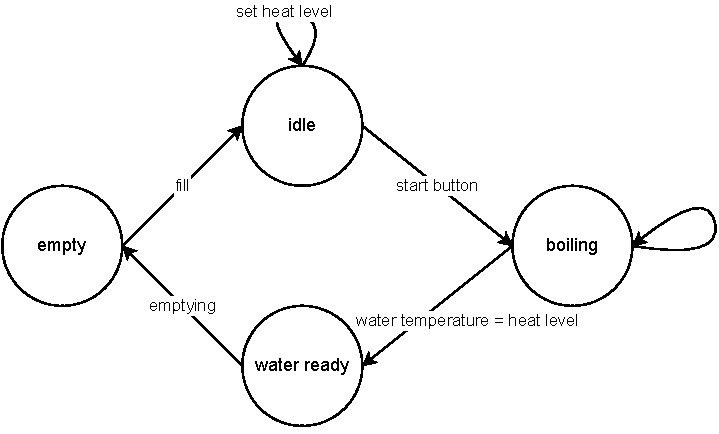
\includegraphics[width=\textwidth]{../digitalDesign/lecture7.pdf}
\end{figure}